%OBAL
\thispagestyle{empty}
\begin{center}
  \textsc{ 
    {\Large \school\\ \faculty}
    \vfill
    {\LARGE \title}\\ \vspace{0.5cm}
    {\large \thesis}
  }
\end{center}
\vfill

\begin{flushleft}
  \year\\
  \hspace{0.5cm} \author
\end{flushleft}


%TITULNY LIST
\thispagestyle{empty}
\begin{center}
  \textsc{ 
    {\Large \school\\ \faculty}
    \vfill
    {\LARGE \title}\\ \vspace{0.5cm}
    {\large \thesis}
  }
\end{center}
\vfill

\begin{flushleft}
  \begin{tabular}{@{}ll}
    Study programme: & \studyprogramme \\
    Study field: & \studyfield \\
	  Department: & \department \\
    Supervisor: & \supervisor
  \end{tabular}
  \vspace{1cm}

  \placeandyear\\
  \hspace{0.5cm} \author
\end{flushleft}




%PREHLASENIE
\thispagestyle{empty}
\null
\vfill
\begin{flushleft}
I hereby declare that I have written this thesis by myself, only
with help of referenced literature, under the supervision of my
supervisor.
~\\
~\\
~\\
\end{flushleft}
\begin{flushright}
...............................................~~~~~~~~~~~~~~~~~~
\\
Michal Piovar\v{c}i~~~~~~~~~~~~~~~~~~~~~~~~~~
~\\
~\\
~\\
~\\
\end{flushright}

\shorthandoff{-} %docasne deaktivuje znak '-' v balicku babel
%ZADANIE EN
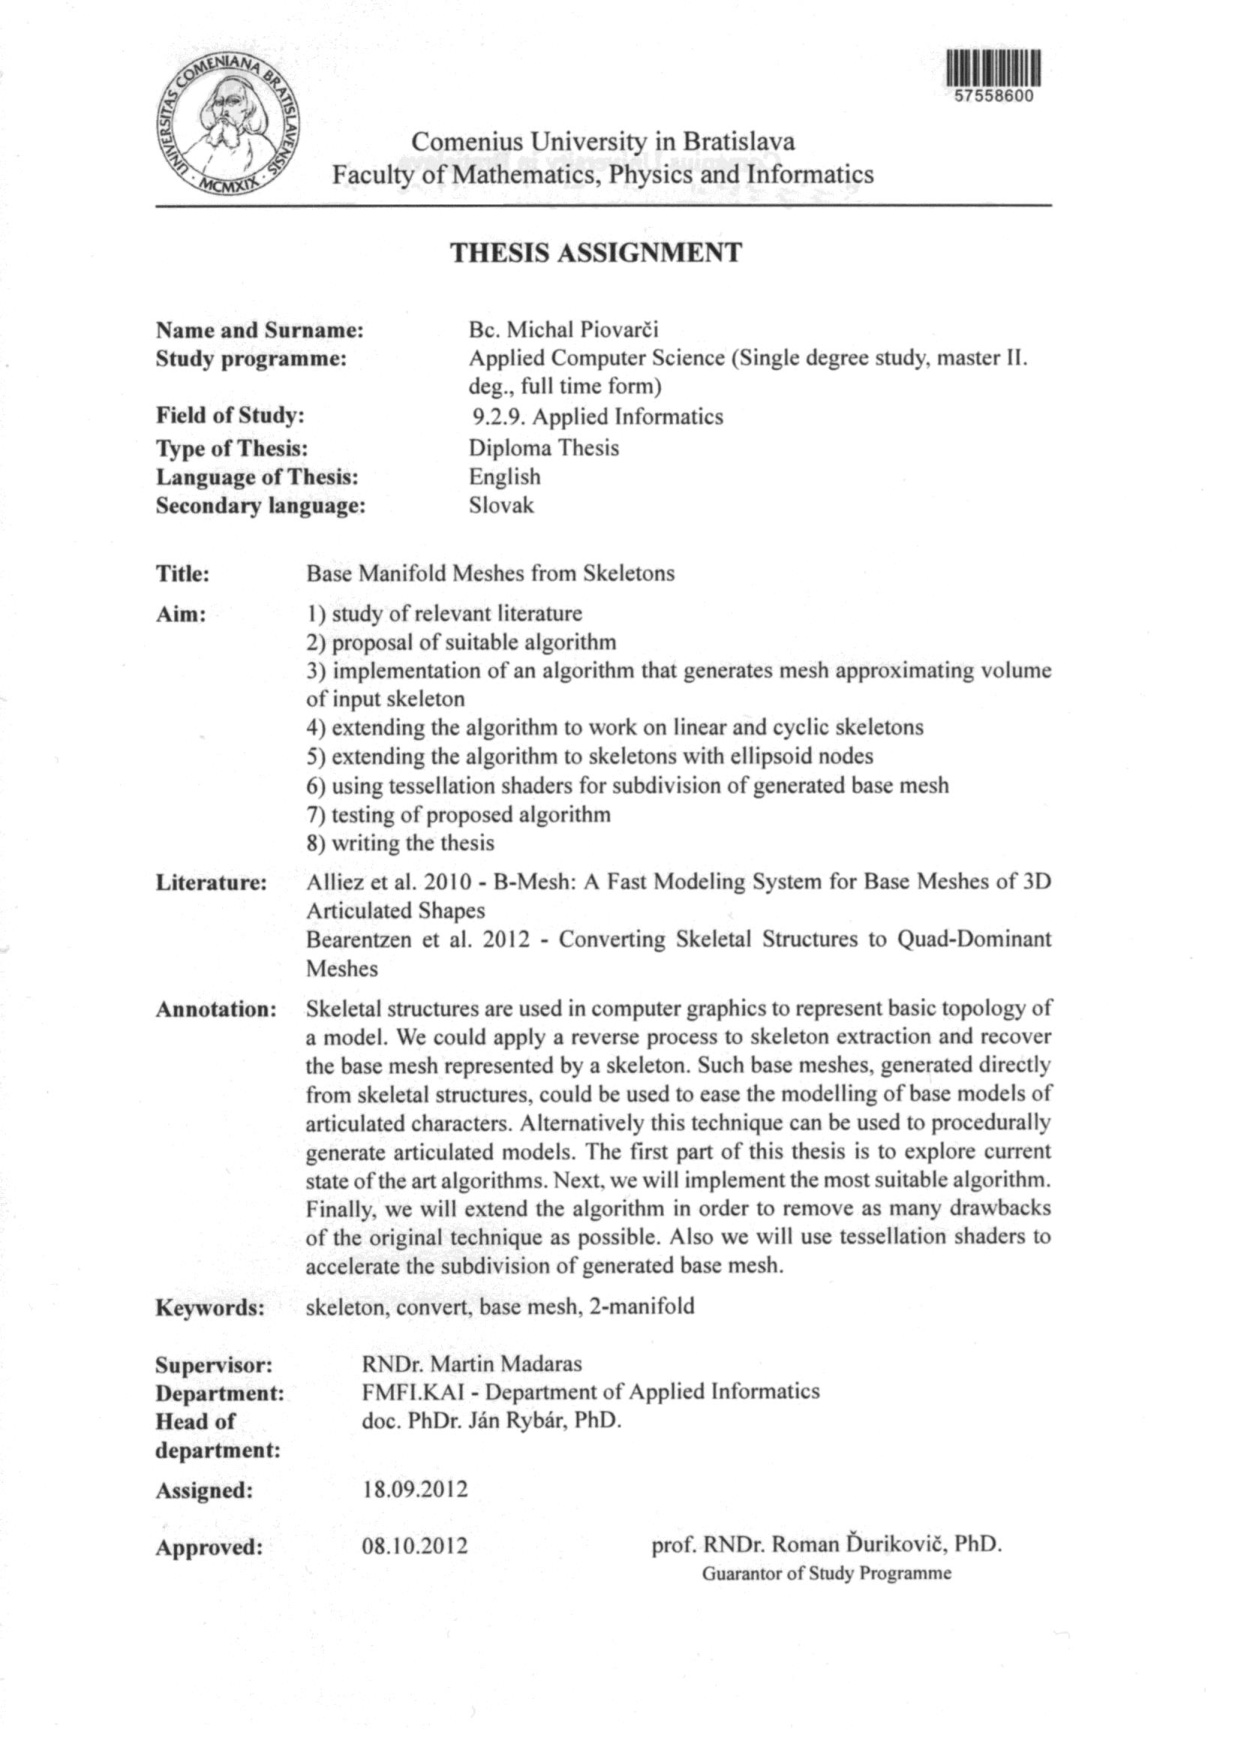
\includepdf[pages=-]{frontmatter/assignement_1.pdf}
%ZADANIE EN 2

\includepdf[pages=-]{frontmatter/assignement_2.pdf}
\shorthandon{-}

%PODAKOVANIE
\chapter{Acknowledgement}
\vfil
\vfil
\vfil
\vfil
I would like to thank my supervisor \supervisor for his help and advices.


%ABSTRAKT EN
\chapter{Abstract}
We have implemented a method, that generates base manifold mesh from an input skeleton, based on Skeleton to Quad Dominant Mesh (SQM) algorithm, which converts skeletons to meshes composed mainly from quadrilaterals.
Each node in skeleton has assigned a sphere.
SQM algorithm first creates branch node polyhedrons for each sphere corresponding to a branch node.
These polyhedrons are bridged with quadrilaterals to create the final base mesh.
We have extended the algorithm to support generation of meshes from cyclic skeletons.
We have also generalized skeleton nodes to ellipsoids instead of spheres.
Finally, we extended the algorithm to generate meshes from linear skeletons without branching and from skeletons, which root node is not a branch node.
The generated base mesh is tessellated on GPU for better visual results.
\\ \\
\textbf{\textsc{Keywords:}} skeleton, convert, base mesh, manifold


%ABSTRAKT SK
\selectlanguage{slovak}
\chapter{Abstrakt}
V tejto práci navrhujeme algortimus, ktorý generuje základné manifoldné meshe zo vstupnej kostry, založený na algoritme Skeleton to Quad Dominant Mesh (SQM), ktorý konvertuje kostry na meshe zložené prevažne zo štvoruholníkov.
Každý vrchol kostry má priradenú guľu.
Algoritmus SQM najprv pre každý vrchol v ktorom sa kostra vetví vygeneruje polyhedrón, aproximujúci guľu príslušného vetviaceho sa vrcholu.
Neskôr sú tieto polyhedróny spojené štvoruholními, čím sa vytvorí základný mesh.
Rozšírili sme SQM algoritmus tak, aby generoval základné meshe aj z cyklických kostier.
Tiež sme zovšeobecnili vstupnú kostru tak, aby bolo možné zadávať elipsoidy namiesto gulí pre každý vrchol.
Nakoniec sme rozšírili algoritmus tak aby vedel generovat základné meshe aj z lineárnych kostier a z kostier, ktorých koreň nie je vetviaci sa uzol.
Vygenerovaný základny mesh teselujeme na grafickej karte, aby sme dosiahli lepsie vizuálne výsledky.
\\ \\
\textbf{\textsc{Kľúčové slová:}} kostra, konverzia, manifold, zakladný mesh

%PREDHOVOR
\selectlanguage{english}
%\chapter{Preamble}
\paragraph{}
Lorem ipsum dolor sit amet, consectetur adipiscing elit. Nunc tristique, sem et feugiat ornare, lorem eros mattis odio, et tempus lectus ipsum nec ante. Phasellus interdum nunc ut sapien semper porttitor. Nam mi erat, faucibus in fermentum eu, varius eu velit. Integer egestas iaculis varius. In pulvinar, ligula eget adipiscing suscipit, nisl ipsum aliquet arcu, eget tristique felis leo vitae magna. Nulla et magna sed justo accumsan ultrices a in leo. Suspendisse tincidunt malesuada leo, eget rhoncus ipsum fringilla at. Integer et tortor vitae nisl fermentum vestibulum. Fusce eu dui neque, a egestas nunc. Vivamus condimentum mi non arcu lacinia et aliquam risus euismod. Nunc ut risus nec elit luctus aliquet et sit amet magna. Vestibulum vehicula enim eget erat fermentum a lacinia purus varius.

\paragraph{}
Duis tempus sem sit amet elit accumsan ultricies. Curabitur a nibh ante, vitae pharetra nulla. Suspendisse non risus elit, in aliquam felis. Maecenas suscipit placerat commodo. Vivamus et molestie odio. Quisque ut augue mi. Quisque aliquam luctus est, ac dignissim ante adipiscing eget. Quisque volutpat, sem vitae placerat condimentum, nunc lorem malesuada leo, sit amet pretium nisi felis nec lorem. Pellentesque nisi ipsum, vestibulum sed lacinia sed, condimentum a turpis.

\paragraph{}
In posuere convallis lectus vel hendrerit. Cras suscipit mi risus. Cum sociis natoque penatibus et magnis dis parturient montes, nascetur ridiculus mus. Donec ante nunc, cursus ac vulputate at, bibendum eget nisi. Nunc eget nunc sed massa blandit posuere id vel quam. Duis bibendum orci vel ligula tempor condimentum. Nulla pharetra tortor at risus dignissim fringilla. Nullam ac massa et nibh auctor vestibulum quis vitae ligula. Suspendisse ultrices eros sit amet lectus dictum dapibus. Sed congue, turpis nec aliquam fermentum, diam nisi cursus nibh, id vulputate massa tellus sit amet turpis.


%OBSAH
\newpage% or \cleardoublepage
% \pdfbookmark[<level>]{<title>}{<dest>}
\pdfbookmark[0]{\contentsname}{toc}
\tableofcontents

%ZOZNAM ILUSTRACII
\listoffigures

%ZOZNAM TABULIEK
\listoftables
